
\PassOptionsToPackage{table}{xcolor}
\documentclass[utf8]{beamer}

\usepackage[T1]{fontenc}
\usepackage[french]{babel}
\usepackage{listings}
\usepackage{multicol}
\usepackage{tikz}
\usepackage{bibentry}

\setbeamertemplate{bibliography item}[text]
\setbeamertemplate{navigation symbols}{}
\usetheme{Amsterdam}

\usetikzlibrary{calc}
\tikzstyle{item}=[rectangle,rounded corners=3pt,thick, dashed, color=beamer@blendedred, fill=gray!20]
% Romain
\newcommand{\cRM}[1]{\MakeUppercase{\romannumeral #1}}  % Capital
\newcommand{\cRm}[1]{\textsc{\romannumeral #1}} % Petit majuscule
\newcommand{\crm}[1]{\romannumeral #1}
% Siècle %
\newcommand{\siecle}[1]{\cRM{#1}\textsuperscript{e}~siècle}

\definecolor{keywords}{RGB}{255,0,0}
\lstset{language=[LaTeX]TeX,
texcsstyle=*\color{keywords},
breaklines=true,
keywordstyle=\color{keywords},
commentstyle=\color{darkgreen},
tabsize=2,
backgroundcolor=\color{lightgrey},
escapeinside=||,
morekeywords={*,subsection,make title,tableofcontents,include graphics}
}

%\insertframenumber/\inserttotalframenumber\hskip2ex

\definecolor{lightgrey}{rgb}{0.9,0.9,0.9}
\definecolor{darkgreen}{rgb}{0,0.6,0} 
\rowcolors{1}{gray!25}{white}

\title{Les stratégies militaires dans les Systèmes Multi-Agents}
\author{Chloé Desdouits, William Dyce}
\date{\today}

\AtBeginSection[]{
  \begin{frame}[plain]
  	\frametitle{Sommaire}
  	\tableofcontents[currentsection]
  \end{frame} 
}
%\frame{\sectionpage}

\begin{document}

\frame[plain]{\titlepage}

\begin{frame}[plain]
	\frametitle{Sommaire}
	\tableofcontents
\end{frame} 

\section{Organisations militaires}
\frame{\sectionpage}

\subsection{Hiérarchiques}
\begin{frame}{Structure}

Une force militaire conventionnelle est à un arbre complet où~:
\begin{itemize}
\item Chaque nœud est commandant de ses nœuds fils,
\item Les feuilles correspondent aux soldats.
\end{itemize}

\end{frame}

\begin{frame}{Structure}

\begin{center}
\begin{tabular}{ l | c c }
\cellcolor{white}	& \multicolumn{2}{c}{\textbf{Civilisation}} \\
\textbf{Effectif}	& \textbf{Perse}& \textbf{Mongol} \\
  \hline
  $>10^4$		& -										& \textit{Ordu}			\\
  $10^4$ 		& \textit{Baivarabam} & \textit{Tumen} 		\\
  $10^3$ 		&	-										& \textit{Myangat} 	\\
  $10^2$ 		& \textit{Hazarabam} 	& \textit{Zuut} 		\\
  $10^1$ 		& \textit{Dathabam} 	& \textit{Avaut} 		\\
\end{tabular}
\end{center}

\end{frame}

\section{Stratégies et tactiques}

\begin{frame}

\begin{tikzpicture}
\node[draw,item] (P) at(0,6) {Politique};
\node[draw=none] (Pe) at(6,6) {\begin{quote}“La politique de la guerre c’est tout simplement décider où, quand, comment, avec quels alliés et pourquoi entrer en guerre.”\end{quote}};
\end{tikzpicture}
\pause
\begin{tikzpicture}
\node[draw,item] (S) at(0,3) {Stratégie};
\node[draw=none] (Se) at(6,3) {\begin{quote}“La stratégie militaire est l'art de coordonner -au plus haut niveau de décision- l'action de l'ensemble des forces militaires de la Nation pour conduire une guerre, gérer une crise ou préserver la paix.”\end{quote}};
\end{tikzpicture}
\pause
\begin{tikzpicture}
\node[draw,item] (T) at(0,0) {Tactique};
\node[draw=none] (Te) at(6,0) {\begin{quote}“La tactique est l'art de diriger une bataille, en combinant, par la manœuvre, l'action des différents moyens de combat en vue d'obtenir le maximum d'efficacité.”\end{quote}};
\end{tikzpicture}%
\footlineextra{\cite{military_strategy, tactic, politique_jomini}}
\end{frame}

\begin{frame}
\pgfdeclareimage[width=6cm]{politique}{../ressources/alliances_ww1}
\pgfdeclareimage[width=7.5cm]{strategie}{../ressources/strategy_ww1}
\pgfdeclareimage[width=5cm]{tactique}{../ressources/Battles_of_Charleroi_ww1}
{\centering
\makebox[0pt]{%
\begin{tikzpicture}
\node[] (Si) at(0,-3) {\pgfbox[left,center] {\pgfuseimage{strategie}}};
\node[] (Pi) at(12.6,-2.66) {\pgfbox[right,bottom] {\pgfuseimage{politique}}};
\node[] (Ti) at(12.6,-5.7) {\pgfbox[right,center] {\pgfuseimage{tactique}}};
\node[draw,item] (P) at(5.5,0.4) {Politique};
\node[draw,item] (S) at(8.5,-3.2) {Stratégie};
\node[draw,item] (T) at(5.5,-6.5) {Tactique};
\end{tikzpicture}%
}\par
}
\footlineextra{\cite{ww1, military_strategy, tactic}}
\end{frame}


\subsection{Stratégies}

\begin{frame}
\frametitle{Sun Tzu}
\framesubtitle{Chine (\siecle{6} BC)}
\begin{tikzpicture}[remember picture,overlay]
	\node[anchor=north east,inner sep=0pt] at ($(current page.north east)+(-0.1cm,-0.75cm)$) {
	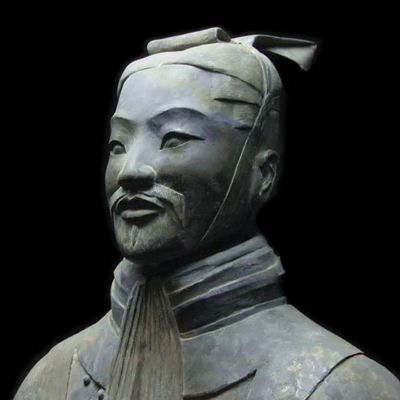
\includegraphics[width=1.9cm]{../ressources/sun_tzu_general}
  };
\end{tikzpicture}
\begin{quote}“L'art de la guerre, c'est de soumettre l'ennemi sans combat.”\end{quote}
\vfill
\begin{columns}[t]
\begin{column}{0.5\linewidth}
Préceptes
\begin{itemize}
\item prendre toutes les possessions de l'adversaire et les conserver intactes
\item adaptabilité, préparation, connaissance du terrain et des forces en présence (espionnage)
\end{itemize}
\end{column}
\begin{column}{0.5\linewidth}
Axes stratégiques
\begin{enumerate}
\item cause morale
\item conditions climatiques
\item conditions géographiques
\item qualités du dirigeant
\item organisation et discipline
\end{enumerate}
\end{column}
\end{columns}

\footlineextra{\cite{tzu1997art, sun_tzu_fighting, sun_tzu_wiki}}
\end{frame}

\begin{frame}{Alexandre le grand}
\framesubtitle{Grèce (\siecle{4} BC)}
\begin{tikzpicture}[remember picture,overlay]
	\node[anchor=north east,inner sep=0pt] at ($(current page.north east)+(-0.1cm,-0.75cm)$) {
	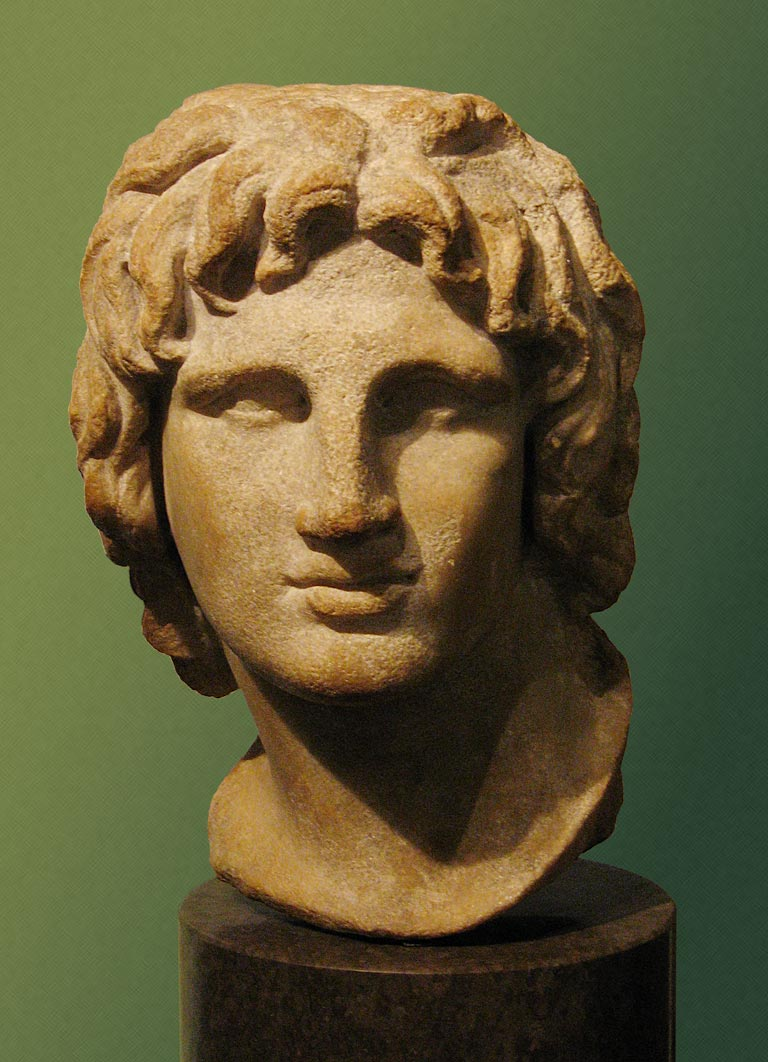
\includegraphics[trim=0cm 8cm 0cm 0cm, clip=true, width=1.9cm]{../ressources/AlexanderTheGreat_Bust}
  };
\end{tikzpicture}
\begin{quote}“Ce qui ne me tue pas me rend plus fort.”\end{quote}
\vfill
\begin{columns}[t]
\begin{column}{0.5\linewidth}
Préceptes
\begin{itemize}
\item conscription et intégration des peuples vaincus
\item allègement de l'équipement des troupes
\end{itemize}
\end{column}
\begin{column}{0.5\linewidth}
Axes stratégiques
\begin{enumerate}
\item assurer ses arrières
\item choisir judicieusement la voie d'accès pour chaque conquête
\end{enumerate}
\end{column}
\end{columns}
\footlineextra{\cite{alexander_the_great, alexandre_balkans}}
\end{frame}

\begin{frame}{Julius Caesar}
\framesubtitle{Italie (\siecle{1} BC)}
\begin{tikzpicture}[remember picture,overlay]
	\node[anchor=north east,inner sep=0pt] at ($(current page.north east)+(-0.1cm,-0.75cm)$) {
	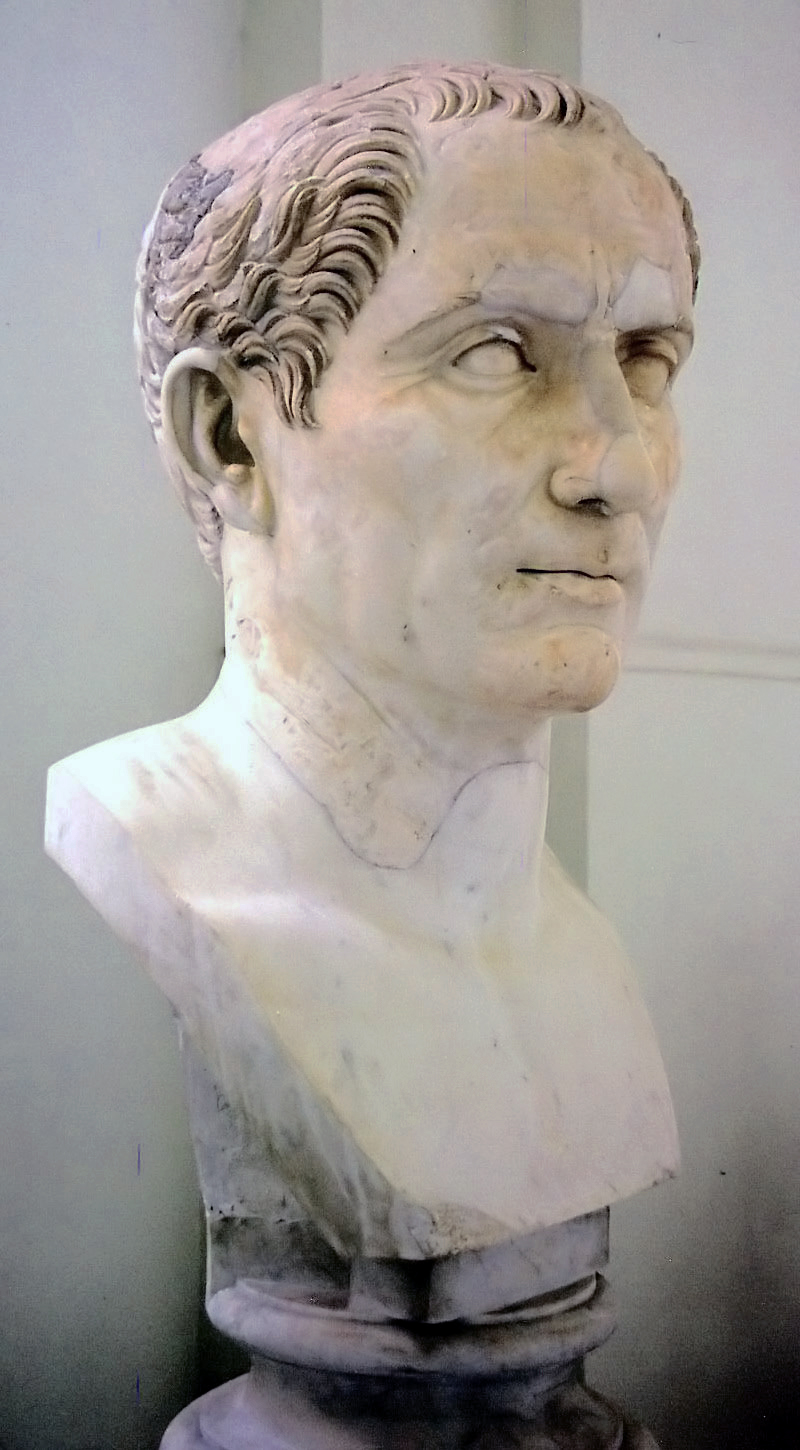
\includegraphics[trim=0cm 20cm 0cm 0cm, clip=true, width=1.9cm]{../ressources/cesare}
  };
\end{tikzpicture}
\begin{quote}“L’expérience, voilà le maître en toutes choses.”\end{quote}
\vfill
\begin{columns}[t]
\begin{column}{0.5\linewidth}
Préceptes
\begin{itemize}
\item stabilité militaire et logistique
\end{itemize}
\end{column}
\begin{column}{0.5\linewidth}
Axes stratégiques
\begin{enumerate}
\item infanterie lourde
\item bataillons étrangers spécialisés
\item formations en fonction des conditions géographiques
\item bivouac fortifié
\end{enumerate}
\end{column}
\end{columns}
\footlineextra{\cite{caesar_wiki, caesar_lacks}}
\end{frame}

\begin{frame}{Genghis Khan}
\framesubtitle{Mongolie (\siecle{12})}
\begin{tikzpicture}[remember picture,overlay]
	\node[anchor=north east,inner sep=0pt] at ($(current page.north east)+(-0.1cm,-0.75cm)$) {
	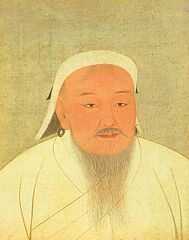
\includegraphics[trim=0cm 1cm 0cm 1cm, clip=true, width=1.9cm]{../ressources/genghis_khan}
  };
\end{tikzpicture}
\begin{quote}“Le plus grand bonheur du Mongol est de vaincre l’ennemi, de ravir ses trésors, de faire hurler ses serviteurs, de se sauver au galop de ses chevaux bien nourris [\ldots]”\end{quote}
\vfill
\begin{columns}[t]
\begin{column}{0.5\linewidth}
Préceptes
\begin{itemize}
\item guerre psychologique
\item règne de la terreur
\item connaissance du terrain : espionnage ; éclaireurs
\end{itemize}
\end{column}
\begin{column}{0.5\linewidth}
Axes stratégiques
\begin{enumerate}
\item peu de troupes ; avant-garde forte
\item troupes montées % logistique et vitesse
\item délégation des décisions
\item relais de communication et ravitaillement
\item attaques biologiques
\end{enumerate}
\end{column}
\end{columns}
\footlineextra{\cite{khan_wiki, military_strategy, mongol_army}}
\end{frame}

\begin{frame}{Napoléon Bonaparte}
\framesubtitle{France (\siecle{18})}
\begin{tikzpicture}[remember picture,overlay]
	\node[anchor=north east,inner sep=0pt] at ($(current page.north east)+(-0.1cm,-0.75cm)$) {
	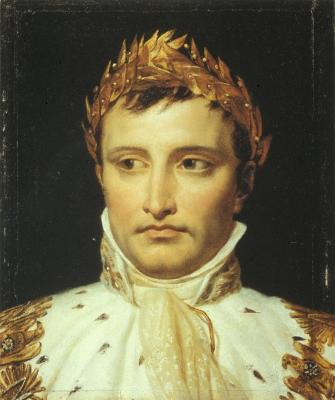
\includegraphics[trim=0cm 2cm 0cm 0cm, clip=true, width=1.9cm]{../ressources/napoleon}
  };
\end{tikzpicture}
\begin{quote}“Réunir ses feux contre un seul point ; une fois la brèche faite, l’équilibre est rompu, tout le reste devient inutile.”\end{quote}
\vfill
\begin{columns}[t]
\begin{column}{0.5\linewidth}
Préceptes
\begin{itemize}
\item recherche systématique de la bataille
\item destruction totale des forces adverses
\item être le plus fort à l’endroit où l’on a décidé de frapper le coup décisif
\end{itemize}
\end{column}
\begin{column}{0.5\linewidth}
Axes stratégiques
\begin{enumerate}
\item vitesse de manœuvre : {\emph Blitzkrieg}
\item fortifications
\item lignes de réapprovisionnement provisoires
\item artillerie
\end{enumerate}
\end{column}
\end{columns}
\footlineextra{\cite{napoleon, napoleon_wiki, napoleon_portrait}}
\end{frame}

\begin{frame}{Synthèse}
%\emph{Consensus sur les points stratégiques suivants :}
%\begin{itemize}
%\item connaissance du terrain et des forces en présence
%\item organisation et discipline
%\item choix politique et géographique de la voie de progression
%\end{itemize}
%\vfill
%\pause
%\emph{Choix stratégiques opposés :}
%
%\bigskip
%\begin{tabular}{rl}
%adaptabilité, délégation, flexibilité & organisation rigide\\
%absorption et intégration de l'adversaire & le détruire et le terroriser\\
%troupes légères et mobiles & troupes lourdes\\
%campements provisoires & fortifications\\
%effectifs réduits & armée expansive\\
%\end{tabular}

\begin{tabular}{|p{0.45\linewidth}|p{0.45\linewidth}|}
\hline
stratégie indirecte & stratégie directe\\
\hline
renseignement & conscription\\
embuscade & recherche de la bataille décisive\\
tromperie & planification et formations\\
sabotage & fortifications\\
\hline
\end{tabular}
   
\end{frame}


\subsection{Tactiques}

\begin{frame}{Manœuvre de flanquement}
\begin{tikzpicture}[remember picture,overlay]
	\node[anchor=north east,inner sep=0pt] at ($(current page.north east)+(-0.1cm,-0.75cm)$) {
	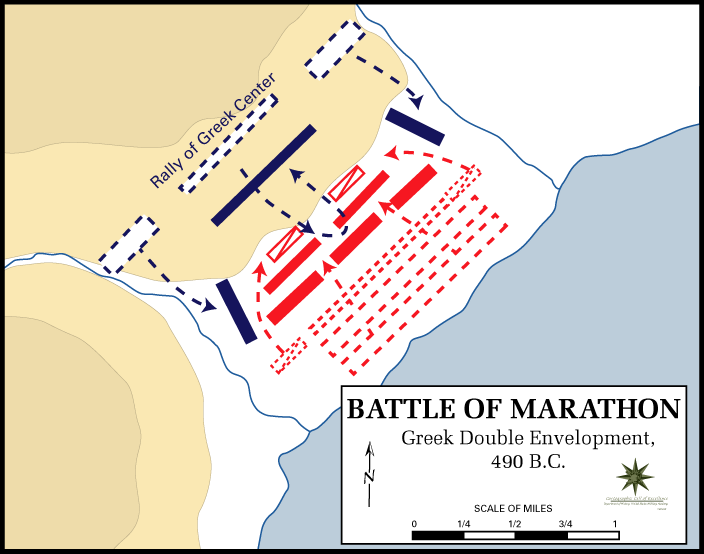
\includegraphics[height=0.5\paperheight]{../ressources/Battle_of_Marathon}
	};
	\node[anchor=south west,inner sep=0pt] at ($(current page.south west)+(0.1cm,0.45cm)$) {
	\fbox{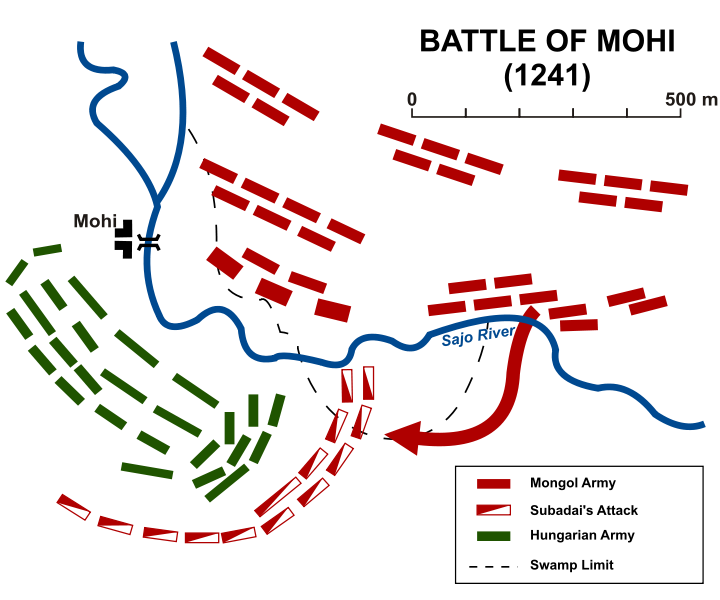
\includegraphics[height=0.53\paperheight]{../ressources/Battle_of_Mohi}}
	};
	\node[draw,item,anchor=north east] at($(current page.north east)+(-0.2cm,-5.7cm)$) {prise en tenaille};
\end{tikzpicture}
\footlineextra{\cite{tactic, flanking_maneuver, pincer_tactic}}
\end{frame}

\begin{frame}{Retraite feinte}

\footlineextra{\cite{mongol_army}}
\end{frame}

\begin{frame}{Le marteau et l'enclume}
\begin{tikzpicture}[remember picture,overlay]
	\node[anchor=north west,inner sep=0pt] at ($(current page.north west)+(1cm,-1.75cm)$) {
	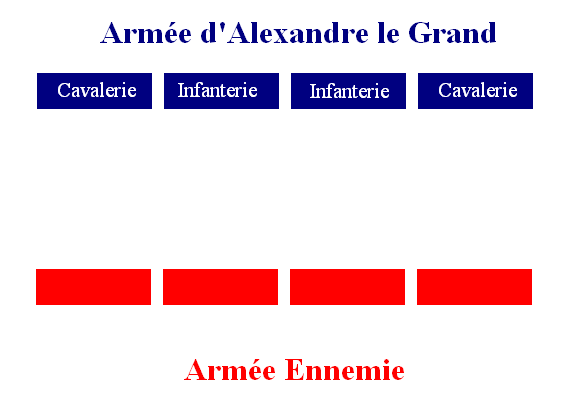
\includegraphics[trim=0.5cm 0.5cm 0.5cm 0.5cm, clip=true, scale=0.25]{../ressources/marteau}
	};
	\node[anchor=north east,inner sep=0pt] at ($(current page.north east)+(-1cm,-1.75cm)$) {
	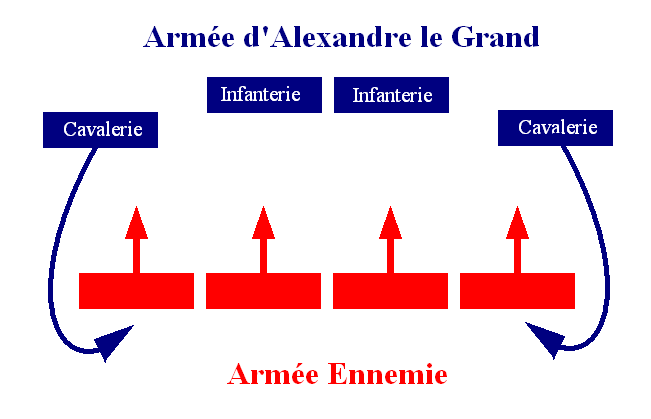
\includegraphics[trim=0.5cm 0.7cm 0.5cm 0.7cm, clip=true, scale=0.25]{../ressources/marteau2}
	};
	\node[anchor=south west,inner sep=0pt] at ($(current page.south west)+(1cm,0.45cm)$) {
	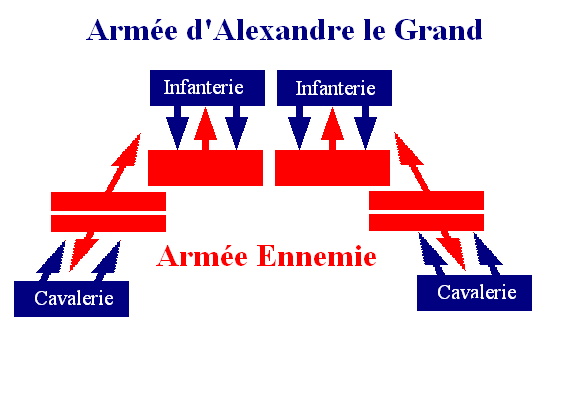
\includegraphics[scale=0.25]{../ressources/enclume}
	};
	\node[anchor=south east,inner sep=0pt] at ($(current page.south east)+(-1.4cm,1.2cm)$) {
	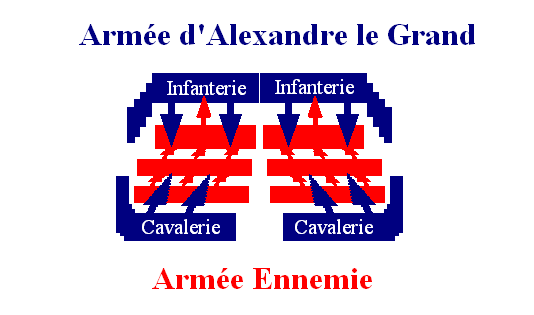
\includegraphics[scale=0.25]{../ressources/enclume2}
	};
\end{tikzpicture}
\footlineextra{\cite{Alexanders_tactics}}
\end{frame}

\begin{frame}{Formation en triple ligne}
\begin{tikzpicture}[remember picture,overlay]
	\node[anchor=north west,inner sep=0pt] at ($(current page.north west)+(2.5cm,-1.6cm)$) {
	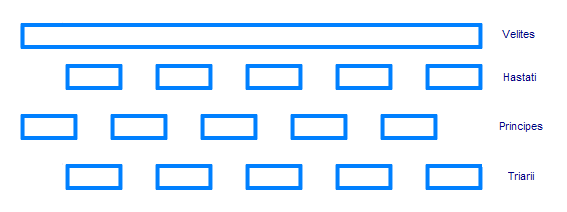
\includegraphics[scale=0.4]{../ressources/Polybian_formation}
	};
	\node[anchor=south west,inner sep=0pt] at ($(current page.south west)+(1.3cm,0.2cm)$) {
	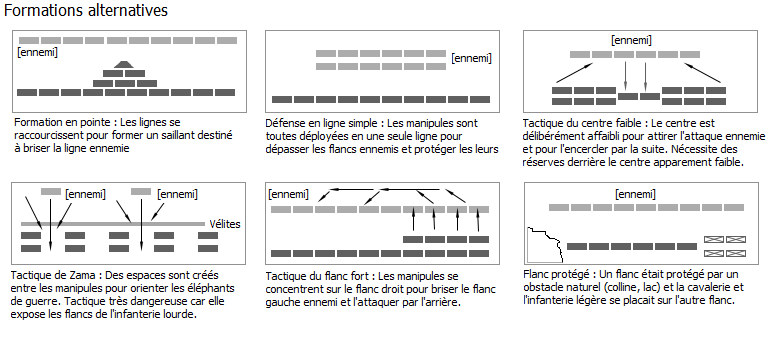
\includegraphics[scale=0.5]{../ressources/Formations_infanterie_romaine}
	};
\end{tikzpicture}
\footlineextra{\cite{roman_infantry_tactics}}
\end{frame}

\begin{frame}{Défense élastique}
\footlineextra{\cite{tactic}}
\end{frame}


\section{Applications aux systèmes multi-agents}


\section{Bibliographie}
\bibliographystyle{plain}
%\bibliographystyle{amsalpha}
\begin{frame}[allowframebreaks]
\frametitle{Bibliographie}
\bibliography{../Bib.bib}
\end{frame}

\end{document}


